\scanpage{3}
% archive foliation: 2
\textbf{Poly-kit}, premier d'une série de jeux éducatifs a obtenu un grand succès dans bon nombre de milieux, auprès de personnes de tout âge, et dans maints pays. \textbf{Lionel March} (Centre for Configurational Studies, Open University, G-B) écrit:

\textit{Le Poly-kit de Janos Baracs remporte un énorme succès dans une école primaire de chez nous. Tous les enseignants en parlent et sa réputation ne cesse de grandir. Je pense moi-même que le Poly-kit pourrait être utilisé lors de nos propres cours donnés à l'Open University.}»

Poly-kit permet de construire tous les polyèdres réguliers et semi-réguliers et certains de leurs duals. (Pour de plus amples informations, voir p. 75 de T.S. n° 1 ou p. 66 de T.S. n° \unsure{3..)|3.)}

Les numéros précédents 1, 2 et 3 publiés en 1979 sont toujours disponibles. Certains articles des numéros 2 et 3 étaient axés sur certains cas spécifiques des domaines de l'architecture et du génie et principalement sur une approche modulaire du design urbain et les systèmes d'immeubles industrialisés. D'autres articles faisaient ressortir les questions mathématiques prédominantes qui se distinguent dans cette recherche.

Déjà, en cette seconde année de publication de la revue, l'échange des résultats de recherche et des problèmes pendants du domaine de la topologie structurale ont atteint un niveau très satisfaisant. Nous sommes très heureux de pouvoir compter sur la collaboration de tant de mathématiciens, architectes et ingénieurs intéressés par le sujet si intrigant et si passionnant qu'est la topologie structurale et de pouvoir ainsi nous adresser à vous directement par le biais du bulletin. Certains d'entre vous peuvent désirer consulter tout simplement Topologie Structurale à la Bibliothèque au lieu de s'abonner personnellement. Dans ce cas, veuillez indiquer sur la carte-réponse ci-dessous que vous aimeriez figurer sur notre liste d'envoi, uniquement pour les nouvelles. Nous désirons maintenir le contact avec vous.

\noindent\dotfill

\noindent N° d'abonné (si nécessaire) \underline{\hspace{1cm}}\hfill\textbf{\Large Topologie Structurale}

Nom et adresse du demandeur:
\begin{center}
\rule{.8\linewidth}{.4pt}\\[1ex]
\rule{.8\linewidth}{.4pt}\\[1ex]
\rule{.8\linewidth}{.4pt}\\[1ex]
\rule{.8\linewidth}{.4pt}\\[1ex]
\rule{.8\linewidth}{.4pt}
\end{center}

Veuillez m'envoyer:
\diagram{\[\begin{array}{llcc}
&&\text{Individuel}&\text{Institution}\\
\square&\text{Abonnement à Topologie structurale pour 1980 (N°s 4-6)}\ \cdots&\$20&\$30\\
\square&\text{Numéros précédents publiés en 1979 (1-3)*}\ \cdots&\$20&\$30\\
\square&\text{Numéro individuel:}\quad\square\ \#1^*\quad\square\ \#2\quad\square\ \#3\ \cdots\ \text{chacun}&\$10&\$15\\
\square&\text{Poly-kits. Combien?}\ \underline{\hspace{1cm}}\ \cdots\ \text{chacun}&\$10&\$10\\
&\hfill\text{*si disponible}&&
\end{array}\]}

$\square$ Veuillez m'inscrire sur votre liste d'envoi pour les nouvelles.\\
$\square$ Montant total joint:\underline{\hspace{1cm}} s.v.p. établir vos chèques au nom de «Topologie Structurale».\\
$\square$ Veuillez me facturer.

\noindent\textbf{\Large Adresser à}\hfill
\begin{tabular}{c}
Topologie Structurale, Ecole d'Architecture, Université de Montréal\\
Montréal, Québec, H3C 3J7, Canada
\end{tabular}

\figure{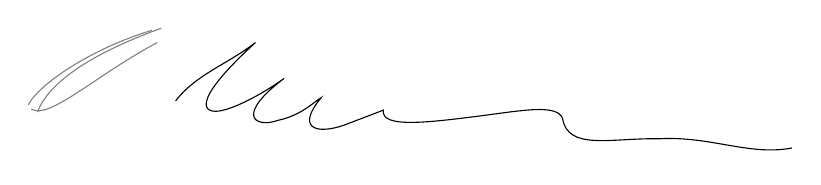
\begin{tikzpicture}[x=.013cm,y=.013cm]
\draw[gray] (0,30) .. controls (10,50) and (61,85) .. (121,103);
\draw[gray] (9,23) .. controls (21,55) and (69,83) .. (130,105);
\draw[gray] (3,26) .. controls (20,15) and (66,59) .. (126,91);
\draw (144,34) .. controls (164,60) and (195,70) .. (222,91) .. controls (166,40) and (166,22) .. (186,24) .. controls (205,27) and (235,45) .. (250,56) .. controls (202,20) and (221,7) .. (244,15) .. controls (267,20) and (279,33) .. (286,37) .. controls (259,4) and (286,1) .. (313,12) -- (347,25) .. controls (344,7) and (391,13) .. (439,19) .. controls (485,25) and (516,31) .. (522,17) .. controls (527,-15) and (570,-2) .. (616,-3) .. controls (666,0) and (705,-20) .. (746,-12);
\end{tikzpicture}}
